
Nei diagrammi di sequenza viene illustrata la sequenza di operazioni necessarie alla realizzazione degli use case del sistema rispetto agli elementi dell'architettura e alle classi di analisi presenti nel sistema.

Gli use case di HBS possono essere categorizzati, a grandi linee, nelle seguenti categorie:
\begin{itemize}
	\item \emph{transazioni}, per gli use case riguardanti le operazioni che i clienti della banca possono effettuare (incluse le operazioni veloci);

	\item interazioni con il sistema di bidding;

	\item operazioni di gestione del sistema di HBS da parte dei dipendenti della banca.
\end{itemize}

\subsubsection{Transazioni}

Gli use case di tipo \emph{transazionale} seguono uno di due modelli:
\begin{itemize}
	\item modello transazionale semplice;

	\item modello transazionale con conferma tramite OTP.
\end{itemize}

In figura~\ref{fig:sequence:transazione:modello} viene indicato il modello transazionale semplice.

\begin{figure*}[h]
	\centering
	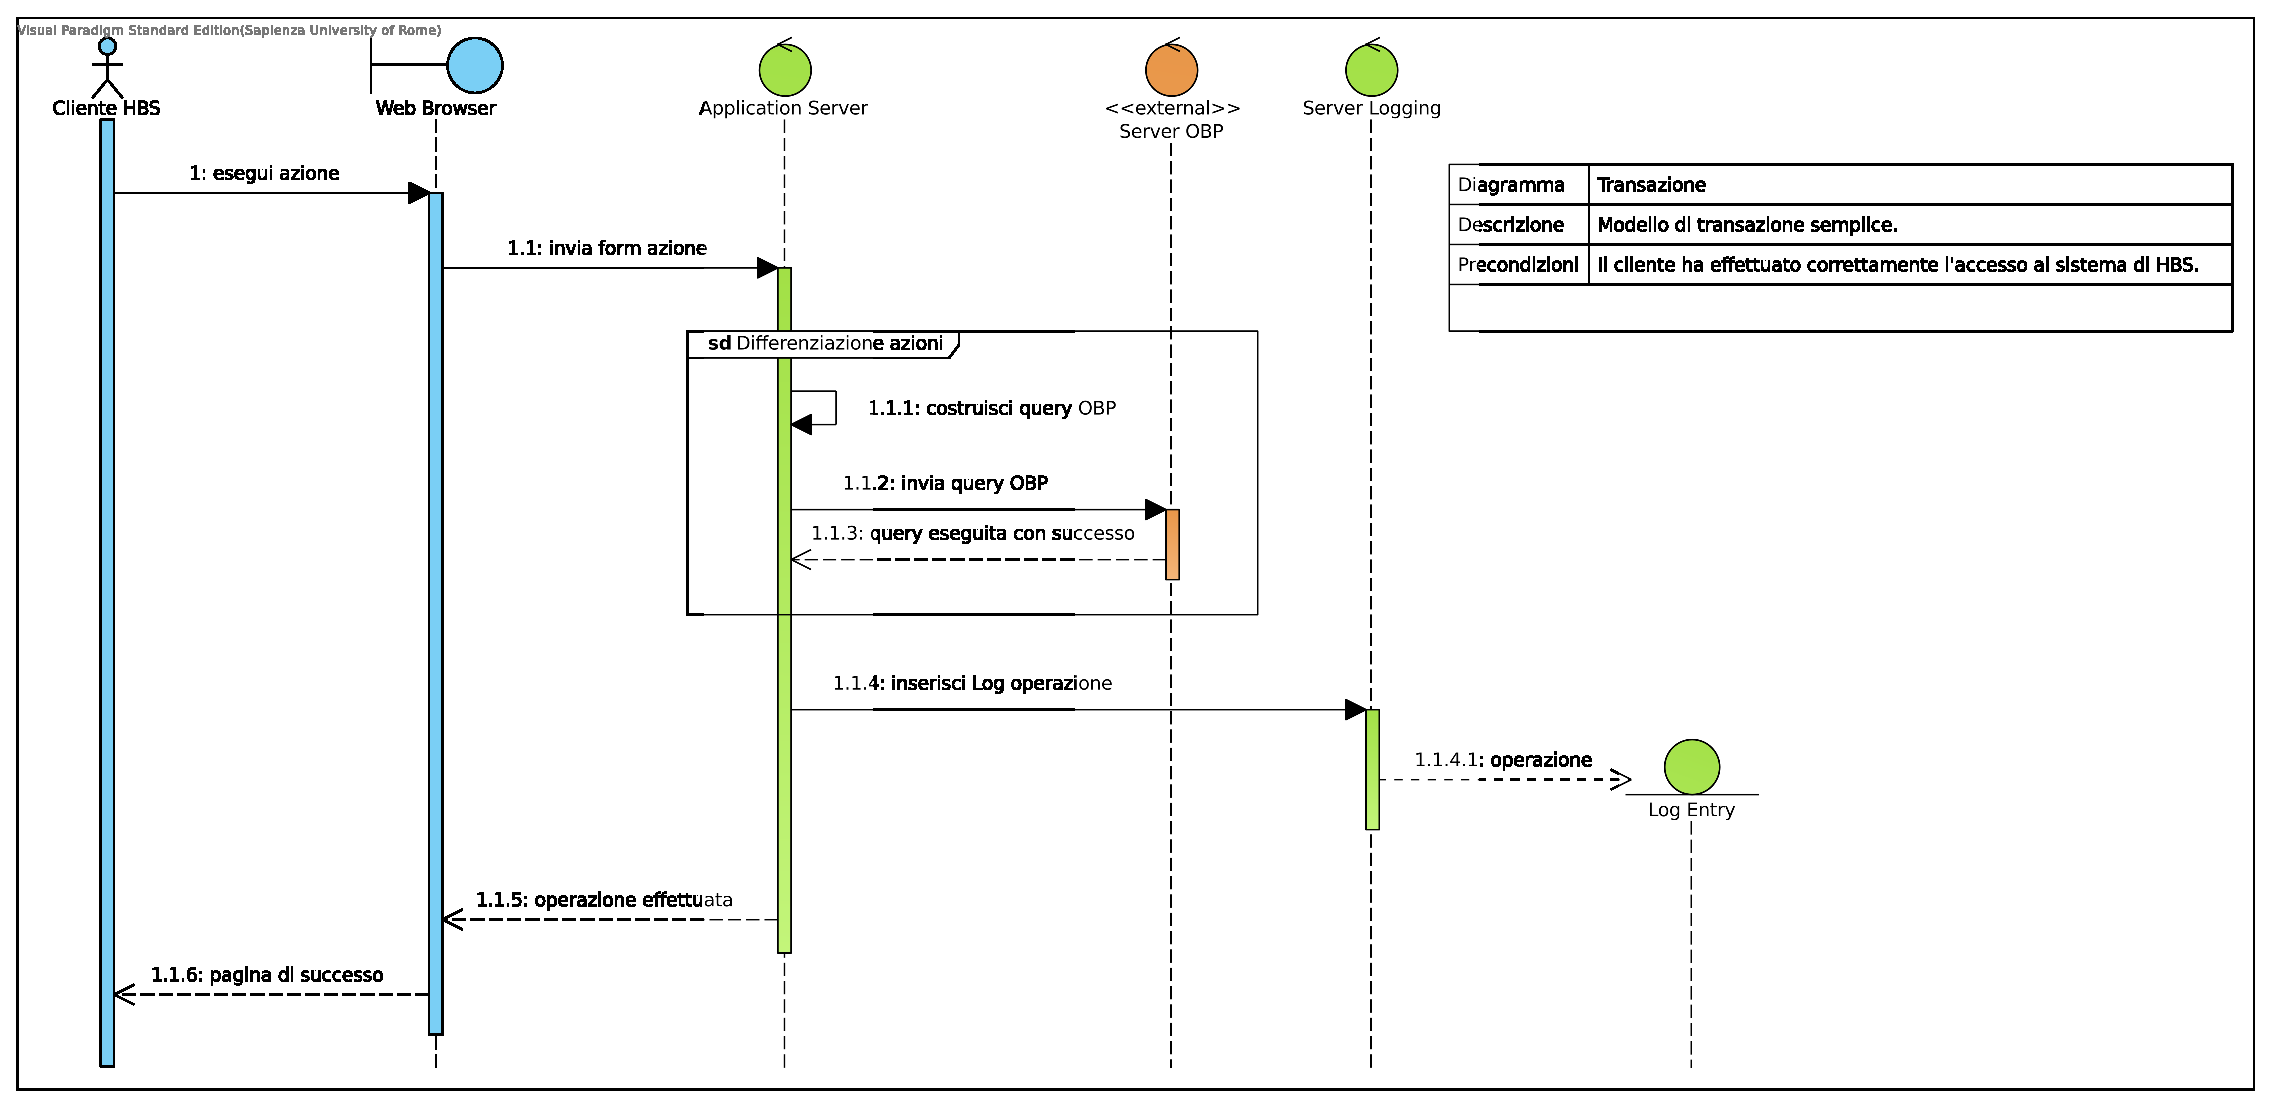
\includegraphics[width=\textheight, angle=90]{Images/sequence/Transazione.eps}
	\caption{Modello di transazione semplice.}
	\label{fig:sequence:transazione:modello}
\end{figure*}

In figura~\ref{fig:sequence:transazione-otp:modello} viene indicato il modello transazionale con conferma tramite OTP.
Use case di questo tipo sono, ad esempio, gli use case riguardanti le operazioni effettuabili da un conto bancario.

\begin{figure*}[h]
	\centering
	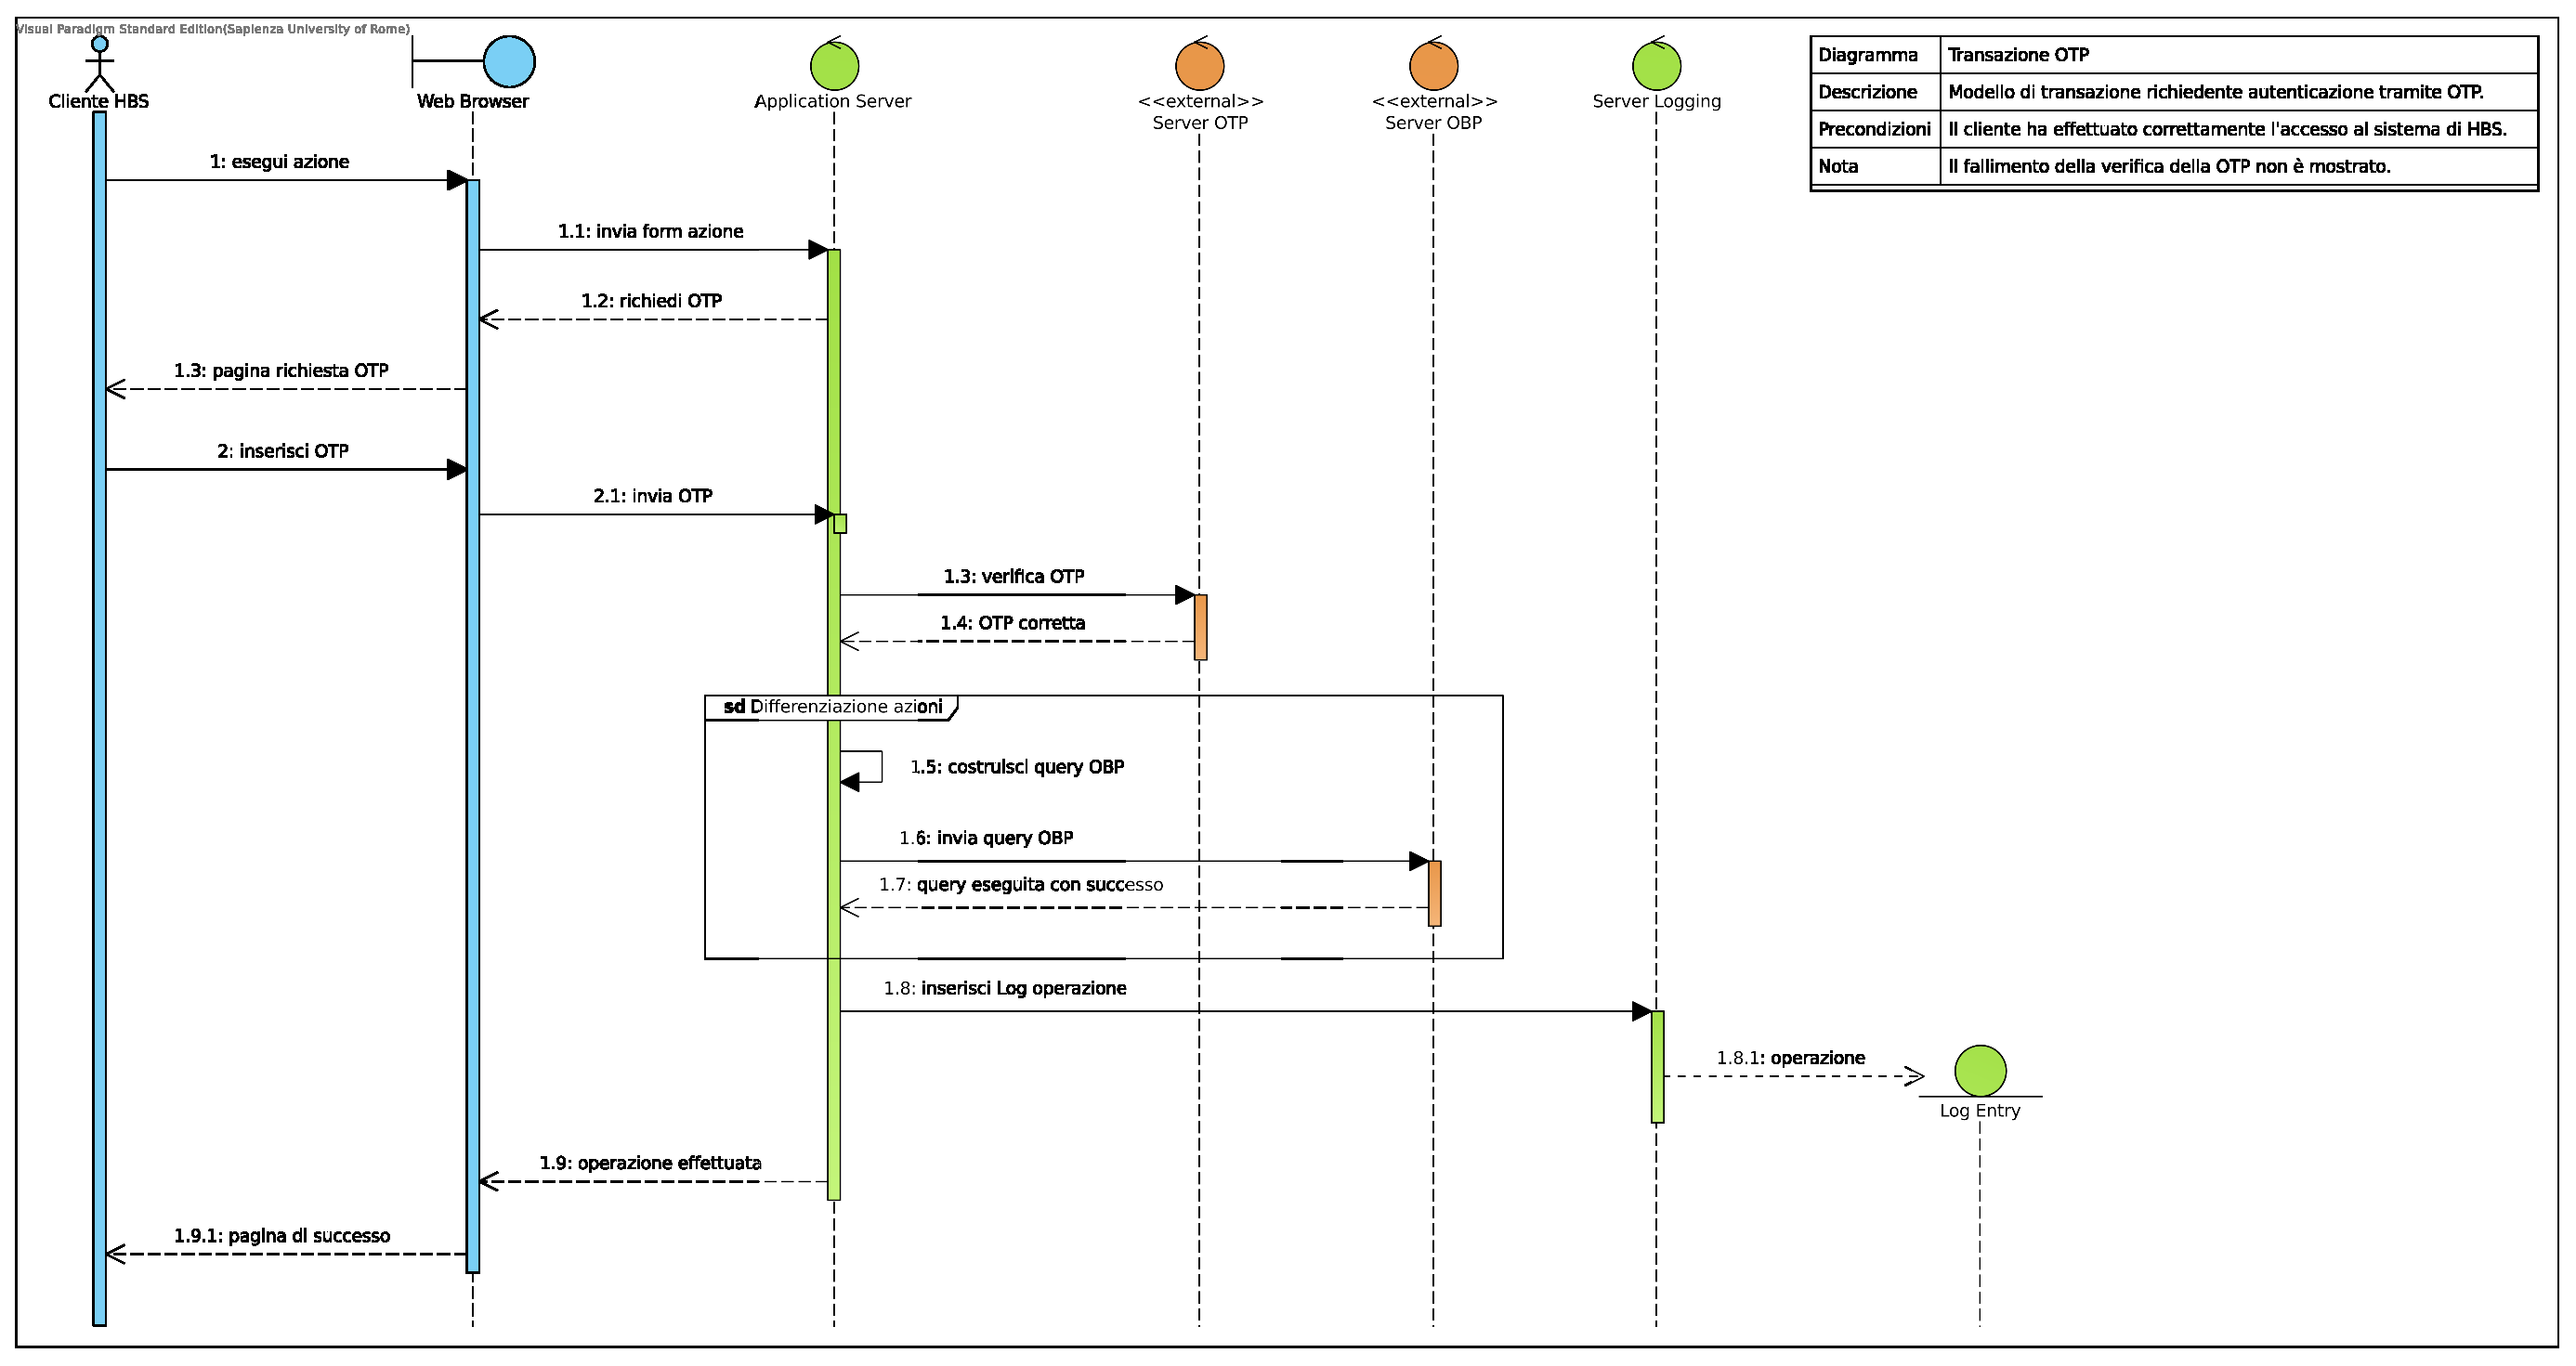
\includegraphics[width=\textheight, angle=90]{Images/sequence/Transazione_OTP.eps}
	\caption{Modello di transazione per la quale è richiesta la conferma tramite OTP.}
	\label{fig:sequence:transazione-otp:modello}
\end{figure*}

\subsubsection{Operazioni}

Le operazioni bancarie effettuabili tramite il sistema di HBS vengono trasmesse da HBS al back-end della banca tramite l'interfaccia di OBP.

Effettuare operazioni veloci (use case \iducDISOPVEL) richiede la creazione di un'operazione ordinaria a partire da un'operazione veloce.
La traduzione da operazione veloce a operazione ordinaria avviene attraverso realizzazioni dell'interfaccia di Traduzione Operazione Veloce.
Ciascun parametro dell'operazione veloce viene tradotto in un parametro dell'operazione ordinaria.
In figura~\ref{fig:sequence:operazione-veloce} viene illustrata la traduzione di un'operazione veloce in un'operazione ordinaria.
Il diagramma di sequenza in figura~\ref{fig:sequence:operazione-veloce} si inserisce nel modello di transazione con conferma tramite OTP illustrato in figura~\ref{fig:sequence:transazione-otp:modello}.

\begin{figure*}[h]
    \centering
    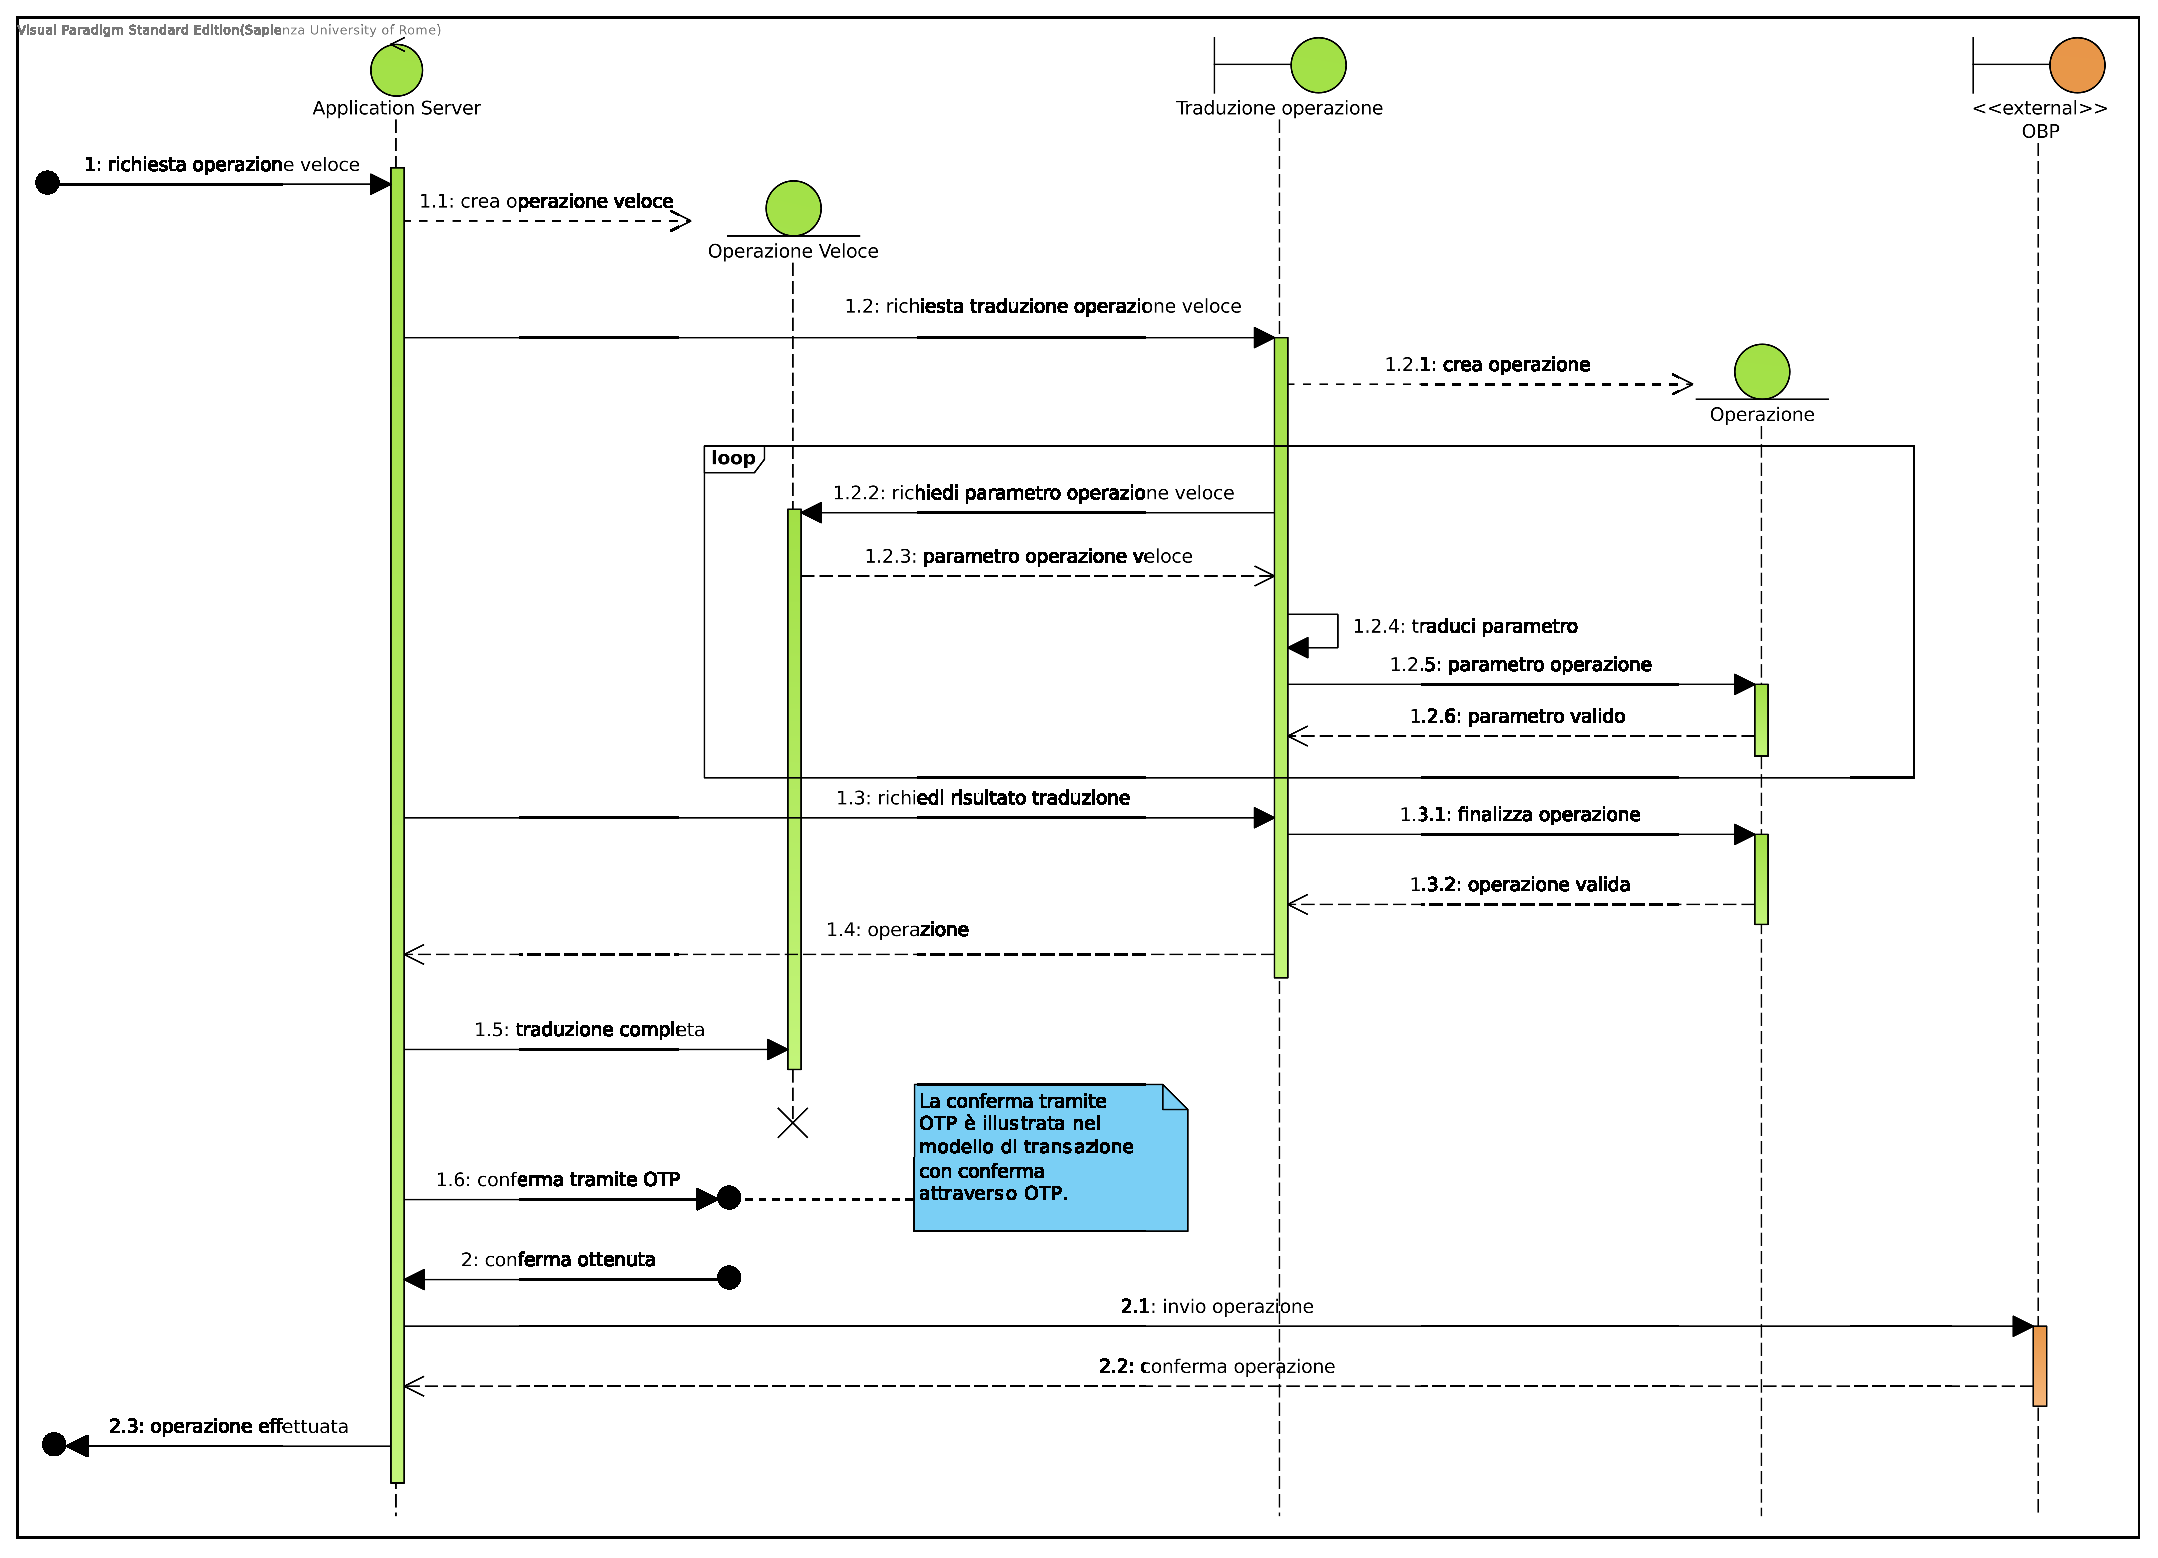
\includegraphics[height=\textwidth, angle=90]{Images/sequence/Operazione_Veloce.eps}
    \caption{Traduzione di un'operazione veloce in un'operazione ordinaria.}
    \label{fig:sequence:operazione-veloce}
\end{figure*}

\subsubsection{Dipendenti}

I casi d'uso relativi ai dipendenti della banca riguardano compiti di ordinaria amministrazione quale l'iscrizione di nuovi clienti, e compiti propri del sistema di HBS quale la gestione del sistema di bidding da parte dei manager o la gestione delle operazioni veloci da parte dei dipendenti.

In figura~\ref{fig:sequence:crezione-operazione-veloce} viene illustrata la procedura di creazione di un'operazione veloce da parte di un dipendente di HBS.

\begin{figure*}[h]
    \centering
    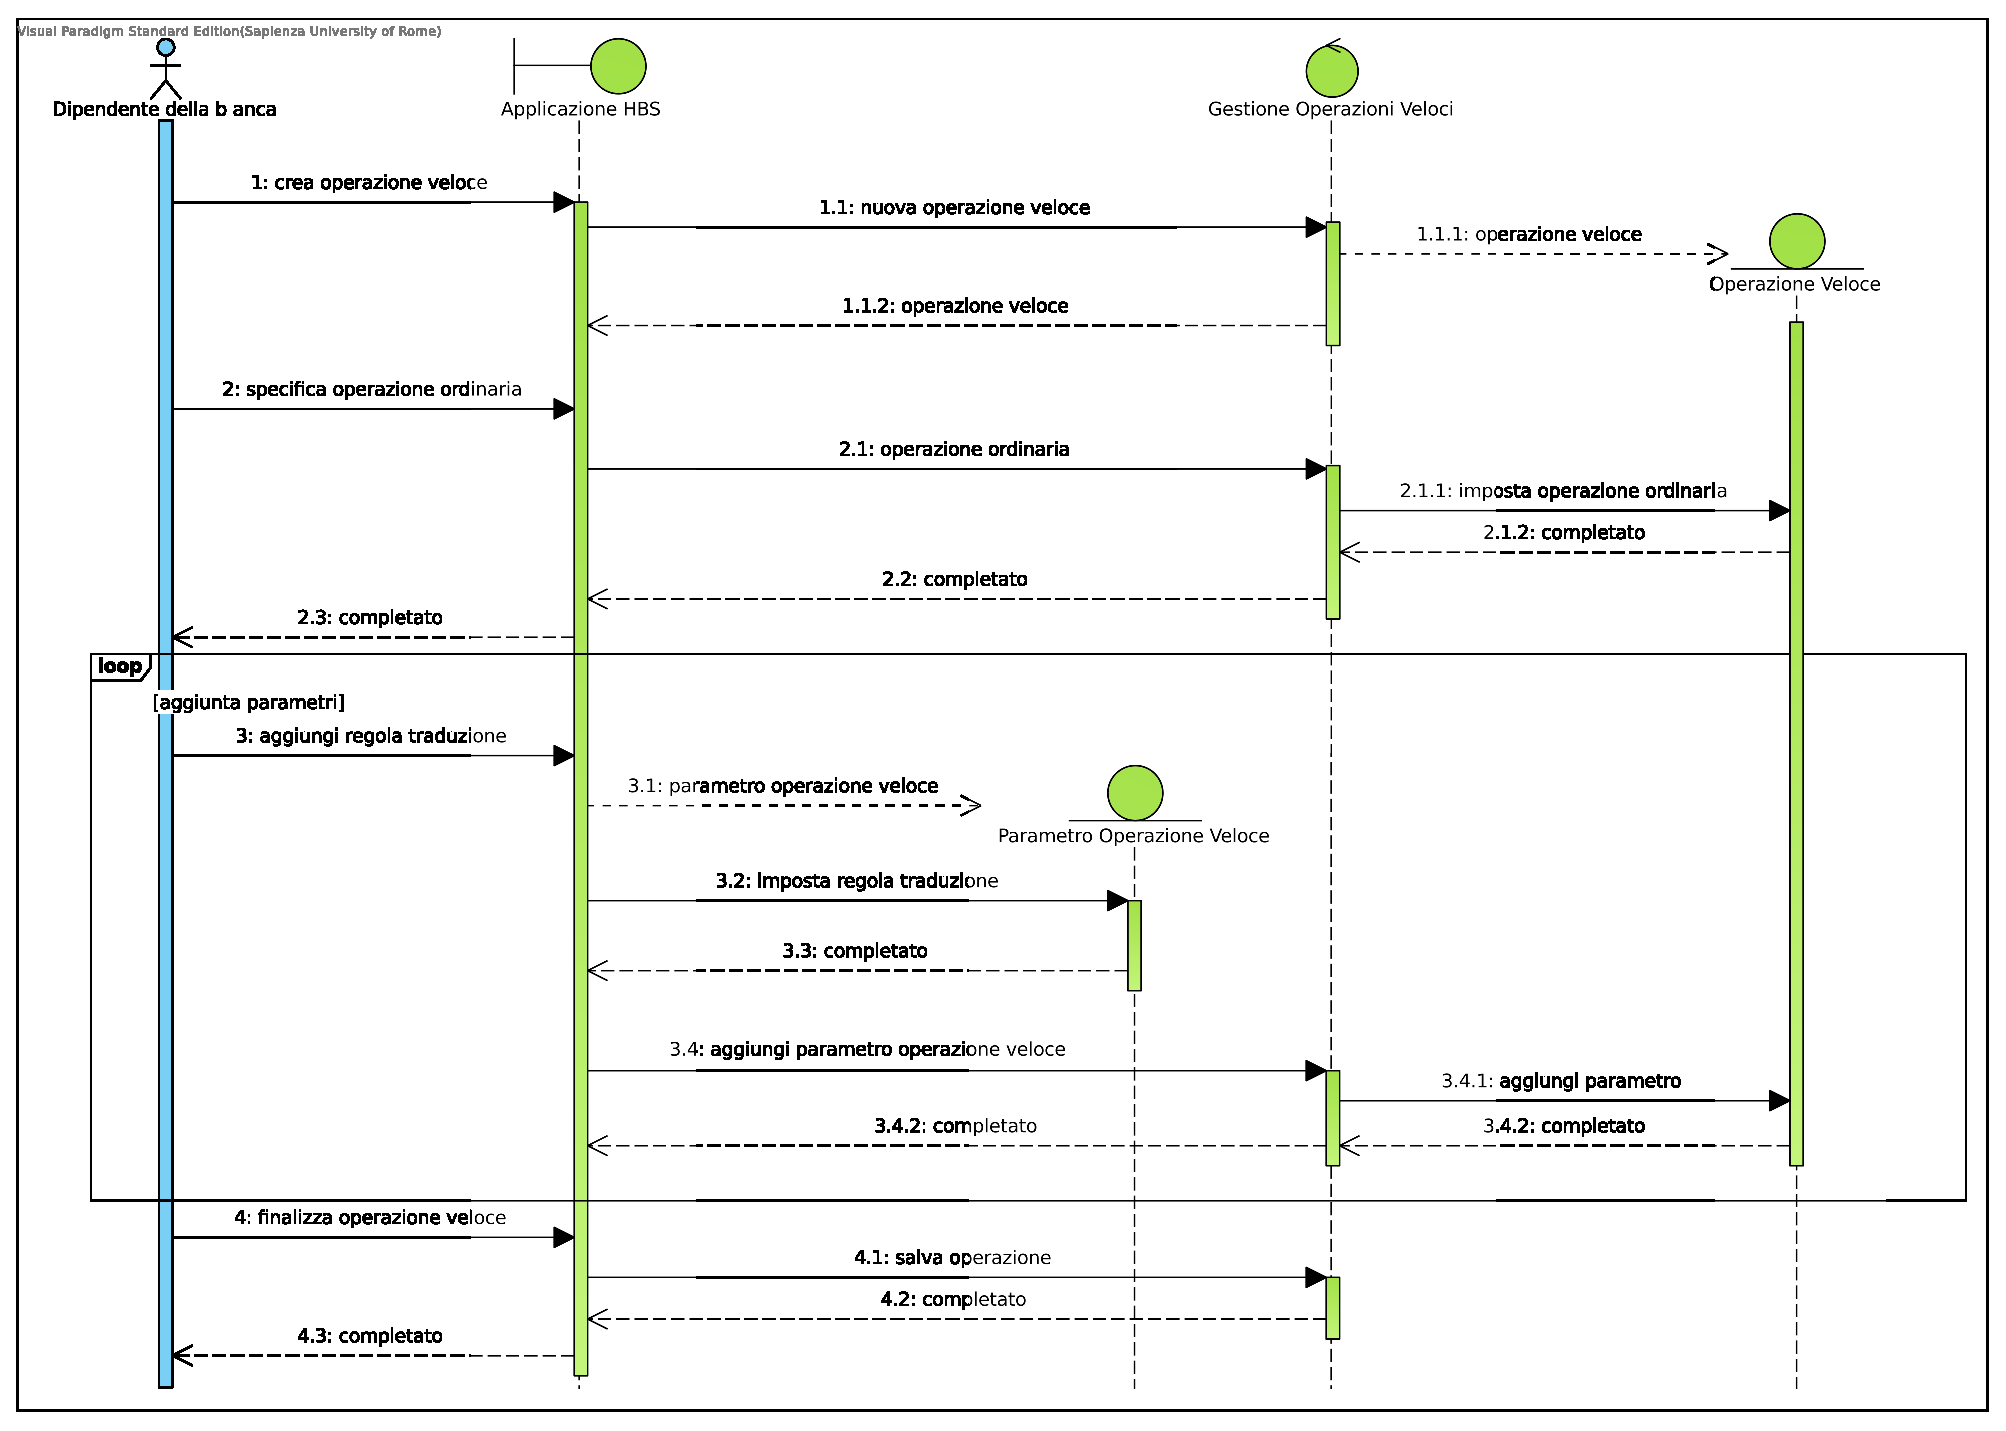
\includegraphics[height=\textwidth, angle=90]{Images/sequence/Creazione_Operazione_Veloce.eps}
    \caption{Creazione di un'operazione veloce da parte di un dipendente della banca.}
    \label{fig:sequence:crezione-operazione-veloce}
\end{figure*}
